\documentclass{article}
\usepackage{authblk}
\usepackage{amsmath}
\usepackage{todonotes}
\usepackage{amssymb}
\usepackage{subcaption}
\usepackage[normalem]{ulem}
\usepackage{graphicx}
\usepackage{cite}
\usepackage{marginnote}
\usepackage[colorlinks=true,urlcolor=blue,citecolor=red,linkcolor=red,bookmarks=true]{hyperref}
\usepackage{soul}
\usepackage{pgfplots}
\pgfplotsset{compat=1.14}
\usepackage{tikz}
\usetikzlibrary{arrows.meta,shapes.geometric} 
\usepackage{float}
\usepackage{geometry}
\hypersetup{linkcolor=red,citecolor=green,urlcolor=blue}  


\newcommand{\fp}{P_{\text{fp}}}
\newcommand{\fn}{P_{\text{fn}}}
\newcommand{\Se}{S_\text{e}}
\newcommand{\Sp}{S_\text{p}}
\newcommand{\mi}{S_{\text{fn}}}
\newcommand{\err}[1]{E_{\text{{#1}}}}%_{\text{rel}}}
\newcommand{\eff}[1]{E_{\text{{#1}}}}%_{\text{rel}}}
\renewcommand\Affilfont{\itshape\small}
\renewcommand{\Pr}{\mathbb{P}}
\newcommand{\data}{\mathbf{d}}
\newcommand{\sens}{S_{\text{e}}}
\newcommand{\spec}{S_{\text{p}}}
% \newcommand{\tn}{P_{\text{tn}}}


\begin{document}
\title{An Accurate Model for SARS-CoV-2 Pooled RT-PCR Test Errors}

\author[1,2]{Yair Daon}
\author[1,3,*]{Amit Huppert}
\author[1,2,*]{Uri Obolski}

\affil[1]{School of Public Health, The Faculty of Medicine, Tel Aviv
  University\\ Tel Aviv, Israel}

\affil[2]{Porter School of the Environment and Earth Sciences, The
  Faculty of Exact Sciences, Tel Aviv University\\ Tel Aviv, Israel}

\affil[3]{The Biostatistics and Biomathematics Unit, The Gertner
  Institute for Epidemiology and Health Policy Research, Sheba Medical
  Center, Tel Hashomer, 52621 Ramat Gan, Israel}

\affil[*]{Equal contribution}

\date{}

\maketitle

\begin{abstract}
Pooling is a method of simultaneously testing multiple samples for the
presence of pathogens. Pooling of SARS-CoV-2 tests is increasing in
popularity, due to its high testing throughput. A popular pooling
scheme is Dorfman pooling: test $N$ individuals simultaneously, if the
test is positive, each individual is then tested separately;
otherwise, all are declared negative. Most analyses of the error rates
of pooling schemes assume that including more than a single infected
sample in a pooled test does not increase the probability of a
positive outcome. We challenge this assumption with experimental data
and suggest a novel and parsimonious probabilistic model for the
outcomes of pooled tests. As an application, we analyze the
false-negative rate (i.e., the probability of a negative result for an
infected individual) of Dorfman pooling. We show that the
false-negative rates under Dorfman pooling increase when the
prevalence of infection decreases. However, low infection prevalence
is exactly the condition when Dorfman pooling achieves highest
throughput efficiency. We therefore implore the cautious use of
pooling and development of pooling schemes that consider correctly
accounting for tests' error rates.
\end{abstract}
\newpage

\section*{Introduction}
Reverse transcription polymerase chain reaction (RT-PCR) testing is a
key component in the fight against the COVID-19 pandemic. RT-PCR
testing can be performed on individuals suspected of infection and
hence break potential transmission chains. Moreover, in some
countries, RT-PCR testing has become a routine procedure of
surveillance, testing incoming air passengers in airports
\cite{PoolingAirports, TestingAirportsJapan}, schools students
\cite{PoolSchool}, or even the entire adult population
\cite{MassPooling}.

As such, the need for large-scale testing has resulted in the
application of techniques to increase the throughput of RT-PCR tests
\cite{DorfmanYuvalDor, PoolSize30, BayesianDorfman, MatrixPooling,
  LionDorfman, CherifReview}. These techniques, often termed
\emph{pooling}, or group testing, have originated in the 1940's in the
seminal work of Dorfman and his pooling technique
\cite{DorfmanOriginal, DorfmanYuvalDor}. Under Dorfman pooling, one
selects $N$ individuals and performs a single RT-PCR test on their
combined (\emph{pooled}) samples. If the pooled test yields a positive
result, then each individual is retested separately; otherwise,
everyone is declared negative. The throughput efficiency of Dorfman
pooling has been demonstrated empirically \cite{DorfmanYuvalDor} and
its error rates thoroughly investigated \cite{Kim, Simplistic1,
  OptimalDorfmanPool}.
  
The study and practice of pooling has advanced considerably since
Dorfman's original paper, with several other pooling techniques being
applied for SARS-CoV-2.  For example, in \emph{recursive} pooling
\cite{Kim,RecursiveSevenFold}, if the first pooled test is positive,
the pool is split into two and the splitting process
repeats. Otherwise, all pool members are declared negative.  In
\emph{Matrix} pooling \cite{MatrixPooling} a population of size $N=mn$
is arranged in a matrix of dimensions $m\times n$. Each row and column
are then pooled and individuals in the intersection of positive rows
and columns are tested separately. Other, more sophisticated pooling
schemes exist \cite{CompressedPooling}, but studies investigating the
underlying assumptions of pooling are surprisingly lacking.

Studies focused on pooling for SARS-CoV-2 are in a consensus that
sample dilution effects \cite{DilutionHIV, GroupDilution} are not a
concern, even for pools as large as 64 individuals \cite{PoolSize30,
  Lion, DorfmanYuvalDor, DilutionCOVID, CherifReview}. Consequently,
studies assumed that the probability of a true-positive (the test's
\emph{sensitivity}) does not depend on the number of infected samples
in the pool, but rather on the existence of at least one such
sample. Thus, the probability of a positive result in a pooled test
has been (assumed) identical for a pool with one sample from an
infected individual and, e.g., five such samples. This assumption is
common in the group testing literature \cite{Kim, OptimalDorfmanPool,
  CherifReview}, as well as in more specific, SARS-CoV-2 focused
studies \cite{Simplistic1, Simplistic2}. In this study we challenge
this commonly made assumption and demonstrate how using a more accurate
probabilistic model affects the estimation of false-negative rates for
Dorfman pooling.

Several consequences arise from our analysis: Previously estimated
optimal Dorfman pool size \cite{OptimalDorfmanPool} should be
revisited in the case of SARS-CoV-2, as it is influenced by the
prevalence of infection. The error rates of other pooling schemes in
use should also be revisited \cite{BayesianDorfman, Kim}. Another
consequence of our results is that studies that seek precise error
models should be conducted for other pathogens as well, since the
standard error model could prove flawed for other
pathogens. Specifically, all assumptions should be scrutinized,
including (e.g.) the independence of tests, an extremely widespread
assumption in the group testing literature \cite{Kim,
  OptimalDorfmanPool} which dates back to Dorfman's original paper
\cite{DorfmanOriginal}. Finally, new methods should be developed in
order to take advantage of our (and other) more realistic models.

\section*{Methods}
Formally, we consider a pool containing $N$ individuals
$\{1,\dots,N\}$. We denote the true infection state $\theta \in
\{0,1\}^N$, so individual $i$ is infected iff $\theta_i=1$. The RT-PCR
test's sensitivity (true-positive rate) is denoted $\sens$, and the
test's specificity (true-negative rate) is denoted $\spec$. Pooled
test result (data) is denoted $\data \in \{0,1\}$, where $\data=0$ iff
the test returned a negative result.

\subsection*{The common assumption}\label{subsec:common}
Previous studies of pooling schemes assumed that the false-negative
probability does not depend on the number of infected samples, but
merely on the existence of at least one such sample in a pool
\cite{Kim, OptimalDorfmanPool}. Current studies of pooling in the
context of SARS-CoV-2 also employ a similar assumption
\cite{Simplistic1, Simplistic2}. Explicitly, these studies assume:

\begin{align}\label{eq:common}
  \Pr(\data=0|\theta) = 
  \begin{cases} 
    1-\sens & \exists i\ \text{such that } \theta_i = 1\\
    \spec & \text{otherwise}
  \end{cases} 
\end{align}

Below, we refer to equation \eqref{eq:common} as the \emph{common
  assumption}. 

\subsection*{Refuting the common assumption}\label{subsec:refute}
We refute the common assumption with experimental data collected from
\cite{Salazar}, and summarized in Table \ref{table}. There, the
authors investigate Dorfman pooling and, regardless of the pooled test
result, follow up and test each pool member separately. We focus on
128 pools for which at least one subsequent separate test was positive
--- of which 29 pooled tests were negative and 99 positive. In the
data cited in \cite{Salazar}, of the 29 negative pools, subsequent
separate testing yielded a single positive result in 24. In contrast,
of the 99 positive pools, 42 yielded a single positive test upon
subsequent separate testing.

The data in Table \ref{table} allows us to test the following null
hypothesis $H_0$: The probability of a pooled false-negative is equal
for pools with one subsequent positively tested member and pools with
two or more such members. $H_0$ is a direct consequence of the common
assumption, and rejecting $H_0$ implies the common assumption is not
realistic, at least for SARS-CoV-2.

We apply Fisher's exact test for the presence of more than one
positive individual in correctly identified pools. Fisher's test
yields an increased odds ratio of 6.4, 95\% CI (2.2,23.4), with a
p-value $\approx 10^{-4}$. Thus, we reject $H_0$, refuting the common
assumption.

\begin{table}[h]
\centering
\begin{tabular}{ c c c }
                                & Negative pool  & Positive pool \\%& Row total \\ 
\# subsequent positives $=1$    & 24             & 42            \\%& 66        \\  
\# subsequent positives $\geq1$ & 5              & 57            \\%& 62        \\
 Total                          & 29             & 99            \\%& 128 
\end{tabular}
\caption{Contingency table of data from \cite{Salazar}}\label{table}
\end{table}


\subsection*{Our model}\label{subsec:ours}
Since the essence of the refuted common assumption is that
amplification of all samples occurs only once, we assume a more
realistic model: amplification of viral RNA succeeds or fails for each
sample independently. Furthermore, according to \cite{Simplistic1,
  Simplistic2, Kim, OptimalDorfmanPool}, a false-positive does not
depend on the number of negative samples in a pool either. For lack of
data pointing otherwise, we incorporate this assumption into our model
with a small modification. We do assume that a false amplification can
occur only once per pool. However, we also assume false amplification
is independent of any other correct amplification. Specifically, it is
possible that every correct amplification fails \emph{and} an
erroneous one occurs simultaneously. This assumption is somewhat
specific for the current application of screening for SARS-CoV-2 via
RT-PCR. For example, cross-reactivity with other coronaviruses would
have violated this assumption. However, cross-reactivity was ruled out
in \cite{KitComparison}. These assumptions lead to our model, which is
illustrated in Figure~\ref{fig:likelihood} and summarized in equation
\eqref{eq:likelihood}.
\begin{align}\label{eq:likelihood}
    \Pr(\data=0 | \theta) &= \spec\prod_{i=1}^N (1-\sens)^{\theta_i} =
    \spec(1-\Se)^{\sum_i\theta_i}.
\end{align}

\begin{figure}[H]
  \centering
  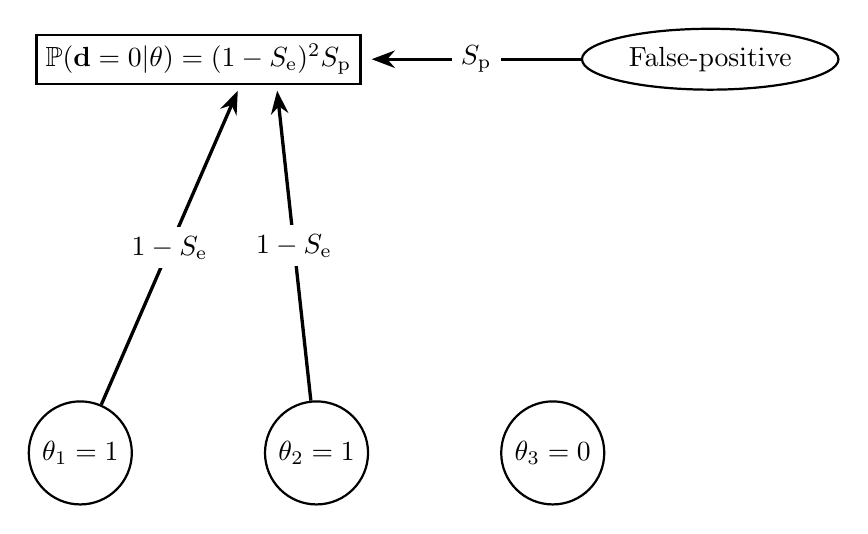
\begin{tikzpicture}
    \begin{scope}[every node/.style={circle,thick,draw}]
      \node[shape=circle,draw=black] (A) at (0,0) {$\theta_1=1$};
      \node[shape=circle,draw=black] (B) at (3,0) {$\theta_2=1$};
      \node[shape=circle,draw=black] (D) at (6,0) {$\theta_3=0$};
      %\node[shape=circle,draw=black] (E) at (6,0) {$\theta_4=1$};

      \node[shape=ellipse,draw=black] (F) at (8,5) {False-positive};
      
      \node[shape=rectangle,draw=black] (G) at (1.5,5)
           {$\Pr(\data=0|\theta)=(1-\sens)^2\spec$};
    \end{scope}

    \begin{scope}[>={Stealth[black]},
        every node/.style={fill=white},
        every edge/.style={draw=black,very thick}]
      \path [->] (A) edge node {$1-\sens$} (2,4.6);
      %\path [->] (B) edge node {$0$} (G);
      %\path [->] (D) edge node {$0$} (G);
      \path [->] (B) edge node {$1-\sens$} (2.5,4.6);
      \path [->] (F) edge node {$\spec$} (3.7,5);
      %\path [-Bar] (D) edge (4.5, 2);
    \end{scope}
  \end{tikzpicture}
  \caption{Illustration of the revised probabilistic model. A pool
    contains individuals $\{1,2,3\}$ with state $\theta=(1,1,0)$
    (i.e., individuals 1 and 2 are infected). A negative pooled test
    ($\data=0$) occurs when three detection paths fail: A
    false-negative occurs for individuals $1$ and $2$, each with
    probability $(1-\sens)$.  Additionally, no false-positive
    detection occurs, with probability $\spec$. Individual $3$ is not
    infected and does not contribute to the probability of the pooled
    test result.}\label{fig:likelihood}
\end{figure}


\subsection*{Application: scheme false-negative rate}
We calculate the false-negative rate for a single \emph{infected}
individual, henceforth referred to as "Donald", under our model and
under the common assumption. We distinguish three types of
false-negative events when performing pooling. A \emph{single test}'s
false-negative is the event of a negative result upon testing Donald
separately, i.e., in an RT-PCR test without pooling. A \emph{pooled}
false-negative occurs when a pooled test containing Donald's sample
(and other samples) yields a negative result, i.e., the pooling fails
to detect at least one positive result. Lastly, a \emph{scheme}
false-negative occurs when an entire pooling scheme fails to identify
Donald as infected. Our first task is to calculate Dorfman's scheme
false-negative rate. Equivalently, we ask: what is the probability of
not identifying Donald as infected under Dorfman pooling?

Denote the prevalence of infection in the (tested) population $q$. We
denote Donald as individual $1$, so that $\theta_1=1$. Then:

\begin{align}
  \begin{split}
    \Pr(\data=0|\theta_1=1) &= \sum_{\theta_2,\dots,\theta_N}
    \Pr(\theta_2,\dots,\theta_N)
    \Pr(\data=0|\theta_1=1,\theta_2,\dots,\theta_N) \\
    %
    %
    %
    &= \sum_{k=0}^{N-1}\Pr\left(\sum_{i=2}^N\theta_i=k\right)
    \Pr\left(\data=0|\theta_1=1,\sum_{i=2}^N\theta_i = k\right)\\
    %
    %
    %
    &= \sum_{k=0}^{N-1}\binom{N-1}{k}q^k(1-q)^{N-1-k} \Sp(1-\Se)^{1+k}\\
    %
    %
    %
    &= \Sp(1-\Se) \sum_{k=0}^{N-1}\binom{N-1}{k}
    \left(q(1-\Se)\right)^k(1-q)^{N-1-k}\\
    %
    %
    %
    &= \Sp(1-\Se)(1-q\Se)^{N-1}. \\
  \end{split}
\end{align}

If the pooled test yields a positive result, Donald is tested
separately. Taking a conservative stand, it is assumed that such a
simple procedure poses no risk of introducing contaminant
RNA. Therefore, the separate test yields a positive result with
probability $\Se$.

We calculate the probability that Donald is mistakenly identified as
not infected, henceforth referred to as the scheme's false-negative
rate and denoted $\mi$. In order to correctly identify an infected
individual as infected, both pooled and separate tests have to yield a
positive result. Thus, the scheme's false-negative rate is:
\begin{align}\label{eq:sfn}
    \begin{split}
        \mi :&= 1 - \Se\Pr(\data=1|\theta_1=1)\\
        %
        &= 1 - \Se\left [1 - \Sp(1-\Se)(1-q\Se))^{N-1}\right].
    \end{split}
\end{align}

\subsubsection*{Comparison metric}
The single test false-negative rate $1-\Se$ and scheme false-negative
rate $\mi$ are compared via:
\begin{equation}\label{eq:erel}
\err{exact} := \frac{\mi - (1-\Se)}{1-\Se} \cdot 100\%.
\end{equation}
$\err{exact}$ is the percentage increase in the pooling scheme
false-negative rate, relative to the single test false-negative rate.

According to the common assumption, the scheme false-negative rate is
$1-\Se^2$. A straight forward calculation shows that this implies the
percentage increase in scheme false-negative rate is $\err{common} :=
100\%\cdot \Se$.

\subsection*{Code Availability}
Code for this manuscript is available at
\url{https://github.com/yairdaon/errorates}.

\section*{Results}\label{section:results}
\subsection*{Scheme false-negative}
We plot $\err{exact}$ for varying prevalence $q$ and sensitivity $\Se$
values, and make the comparison with $\err{common}$. As recommended by
\cite{DorfmanYuvalDor}, we apply different pool sizes $N$, for
different prevalence values. We observe that for a specificity of
$\Sp=0.95$ \cite{DorfmanYuvalDor} and a range of reasonable
sensitivity and prevalence values \cite{KitComparison,
  InterpretingCOVID19Test, EstimatingRatesLourenco,
  FalsePositiveEstimate}, the increase in the scheme false-negative rate
(compared to $1-\Se$), expressed by $\err{exact}$, is at leaset
$60\%$ (Figure \ref{fig1}).

Interestingly, an increase in infection prevalence monotonically
decreases the scheme false-negative rate, as can also be easily seen
from equation \eqref{eq:sfn}. For the chosen parameter ranges, the increase in
the single test false-negative rates increases the relative error
$\err{exact}$. These effects can be seen in Figure~\ref{fig1} (left
panel), upon conditioning on pool size. Extending the range for $\Sp$
yields no qualitative differences. We further compare $\err{exact}$ to
$\err{common}$, showing the discrepancy changes as a function of both
prevalence and the single test sensitivity (Figure~\ref{fig1}, right
panel).
\begin{figure}[H]
  \centering
  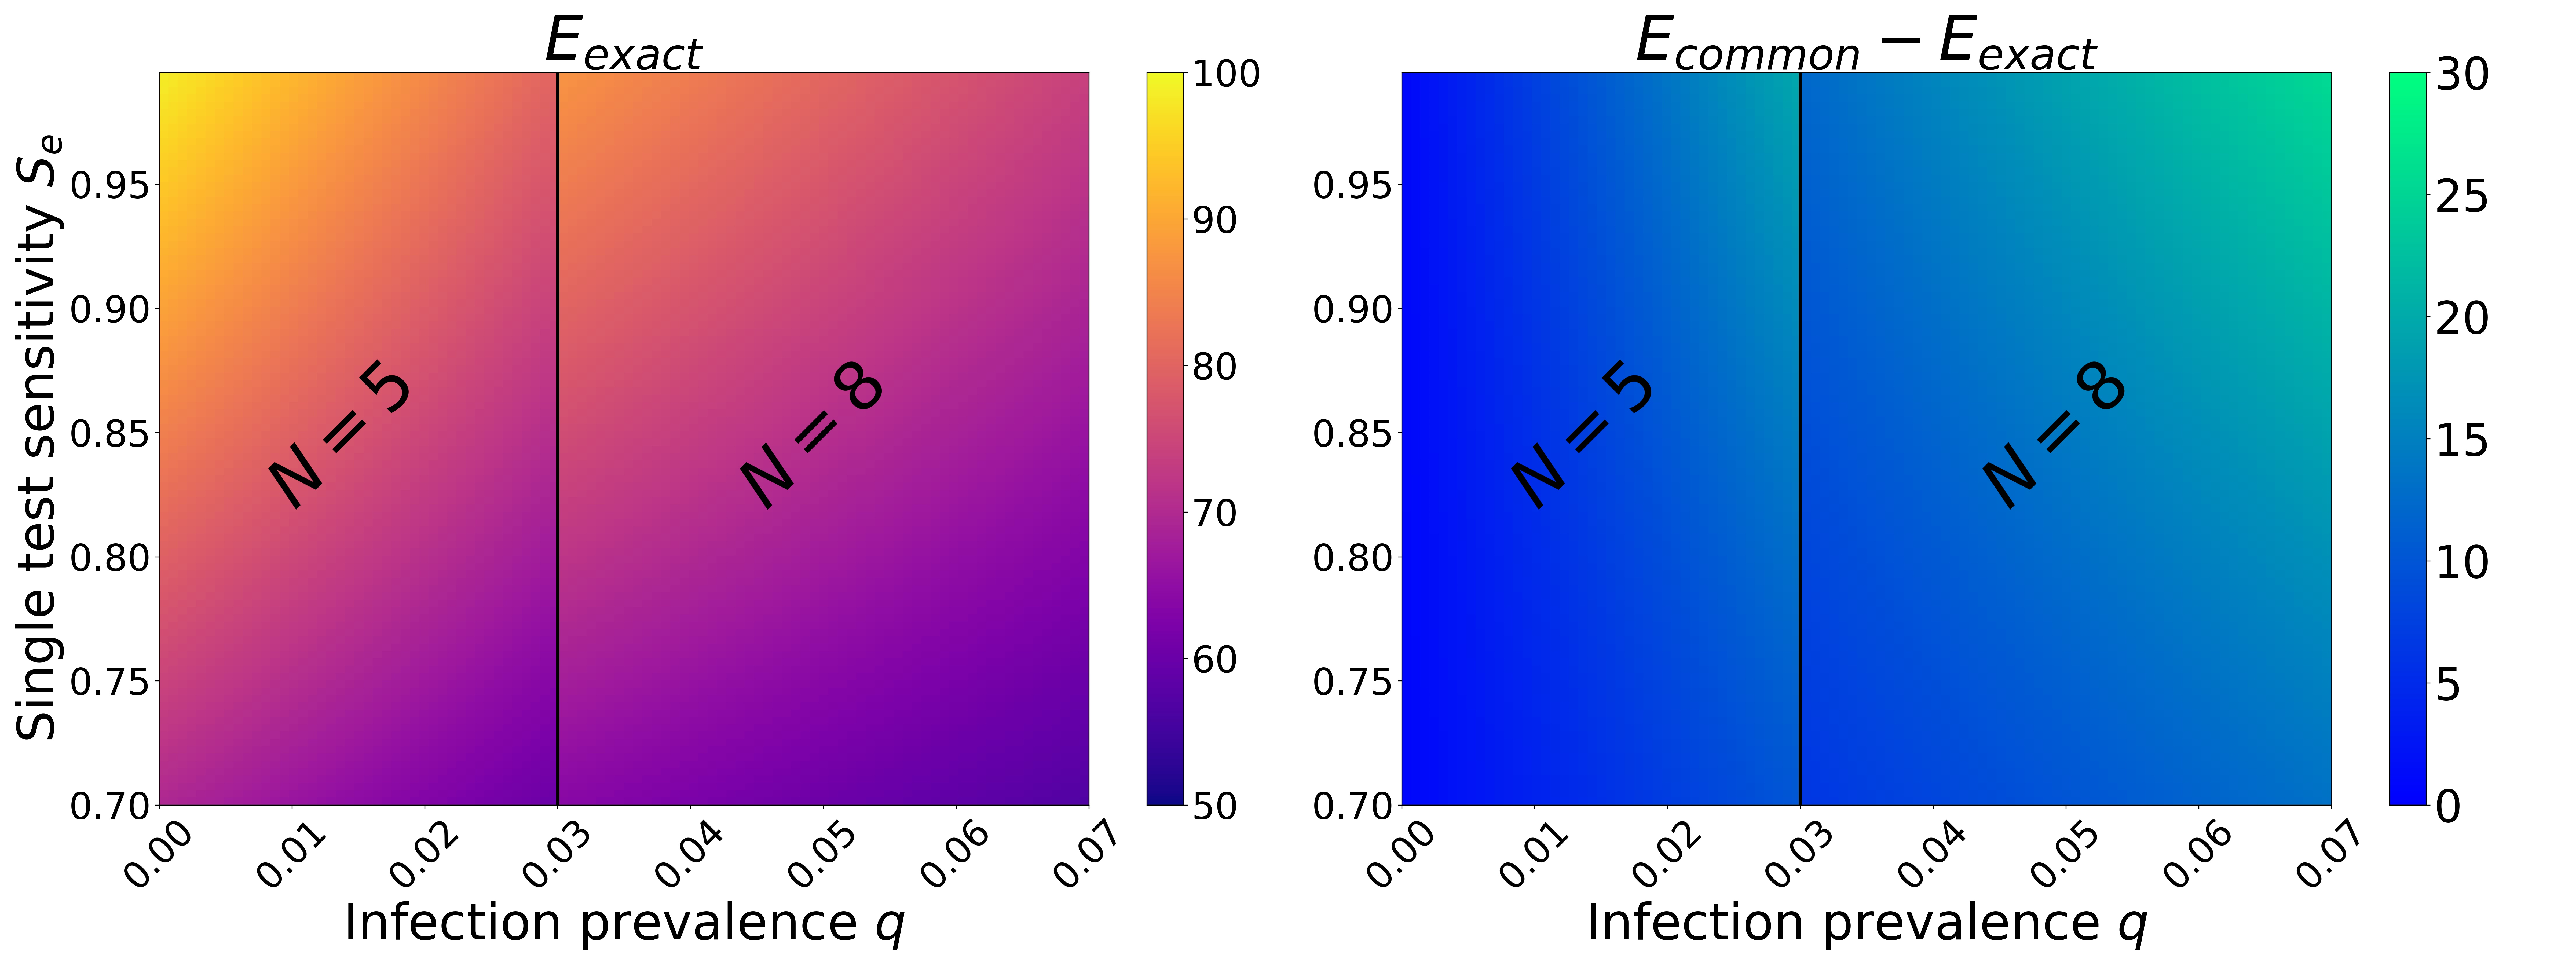
\includegraphics[width=\textwidth]{heatmap_sfn.jpg}
  \caption{Relative increase in Dorfman pooling false-negative rates
    $\err{exact}$. Left: Colors represent $\err{exact}$, the relative
    percentage increase in the scheme false-negative rates relative to
    the single test false-negative rates equation \eqref{eq:erel}. Right:
    colors represent the difference between $\err{common}$ and
    $\err{exact}$. The infection prevalence $q$, is varied on the
    x-axis, while the test sensitivity is varied on the y-axis. Pool
    size $N$, was chosen according to $q$ as in
    \cite{DorfmanYuvalDor}. The left panel shows that $\err{exact}$ is
    largest for low prevalence values $q$. The difference between
    $\err{common}$ and $\err{exact}$ can be as large as 30\%, as seen
    in the right panel. }\label{fig1}
\end{figure}

\section*{Discussion}
In this study, we developed a more realistic and novel probabilistic
model for the outcomes of pooled RT-PCR tests, parameterized for
SARS-CoV-2. Contrary to the common assumption, we assume, based on
data (Table~\ref{table}), that multiple infected individuals increase
the likelihood of a positive pooled test result. A direct consequence
of our model is that low values of infection prevalence increase the
false-negative rates of Dorfman pooling. Importantly, our results
remain qualitatively similar under varying parameter values, in the
observed ranges \cite{KitComparison,EstimatingRatesKucrika,
  EstimatingRatesLourenco, InterpretingCOVID19Test} (Figure
\ref{fig1}). Therefore, our results give rise to a conflict: low
infection prevalence leads to high efficiency of Dorfman pooling
\cite{DorfmanYuvalDor},but also increases false-negative rates.

As the COVID-19 pandemic progresses, the infection prevalence in
various tested populations undergoes frequent changes. Hence, as our
results suggest, pooling schemes employed for mass testing should be
used with caution in populations where infection rates are low. Such
mass-tested populations often include air travel passengers \cite{JTM}
or presymptomatic and asymptomatic individuals \cite{RobinHood}, and
can be crucial for controlling outbreaks \cite{MinaScience}.

Furthermore, an especially important consideration in designing
pooling schemes is explicitly taking into account the intrinsic RT-PCR
error rates . As we have demonstrated above, analyzing the expected
error rates of pooling schemes under a realistic error model is
readily achievable. Designing pooling schemes that optimize testing
while accounting for error rates is, however, considerably more
involved.  Nonetheless, various algorithms explicitly incorporate
error rates into their pooling optimization processes \cite{Kim,
  OptimalDorfmanPool}, including a recent study by our group which
employed the herein described error model \cite{DOPE}.  In our
proposed algorithm, we have used an experimental design criterion to
create an algorithm which iteratively performs pooling, updating its
information based on previous results. In doing so, our pooling scheme
shows potential in terms of both reducing false-negative and
false-positive rates, as well as increasing efficiency, although it
has not yet been implemented in real-world settings.

To conclude, pooling is an important technique that can increase
testing throughput in a cost-effective manner. Nevertheless, care must
be given to pooling schemes' false-negative rates, especially under
low infection prevalence settings.

\section*{Acknowledgements}
Yair Daon was supported by a post-doctoral fellowship from the Tel
Aviv University Center for Combating Pandemics and the Raymond and
Beverly Sackler dean's post-doctoral fellowship.

\bibliographystyle{amsplain}
\bibliography{refs}

\end{document}


%% Todos
%% add refs to dilution and paragraph in start
